%======================================================================
%  UPES  |  School of Computer Science  |  Mid-Sem Assignment Report
%  Template for Design and Analysis of Algorithms (CSEG3053)
%  Student: Sparsh Srivastava | SAP ID: 590022251 | Batch: B17
%======================================================================
\documentclass[11pt,a4paper]{article}

%---------------- Packages ----------------
\usepackage[margin=2.3cm]{geometry}
\usepackage[T1]{fontenc}
\usepackage{amsmath,amssymb}
\usepackage{graphicx}
\usepackage{subcaption}
\usepackage{booktabs}
\usepackage{xcolor}
\usepackage{tikz}
\usetikzlibrary{arrows.meta,positioning,shapes.geometric,calc,decorations.pathreplacing}
\usepackage{pgfplots}
\pgfplotsset{compat=1.18}
\usepackage[ruled,vlined,linesnumbered]{algorithm2e}
\usepackage{listings}
\usepackage[most]{tcolorbox}
\usepackage{qrcode}
\usepackage{fancyhdr}
\usepackage[hidelinks]{hyperref}

\definecolor{upesnavy}{HTML}{1F3864}
\definecolor{guide}{HTML}{EAF1FB}
\definecolor{codebg}{HTML}{F7F7F7}

%================ YOUR DETAILS ================
\newcommand{\studentname}{Sparsh Srivastava}
\newcommand{\sapid}{590022251}
\newcommand{\batch}{B17}
\newcommand{\course}{Design and Analysis of Algorithms (CSEG3053)}
\newcommand{\topic}{Best, Worst and Average Case Analysis}
\newcommand{\animationlink}{https://github.com/SPARSHsrihero1/daa-case-analysis}
\newcommand{\submissiondate}{\today}
%==============================================

\newif\ifshowguidance
\showguidancefalse   % set to \showguidancetrue to see guidance boxes

\newtcolorbox{guidancebox}{colback=guide,colframe=upesnavy!60,
  fonttitle=\bfseries\small,title=Guidance (delete or hide before submitting),
  fontupper=\small,boxrule=0.5pt,arc=2pt}
\newcommand{\frameimg}[1]{\IfFileExists{#1}{\includegraphics[width=\linewidth]{#1}}%
  {\fbox{\parbox[c][0.7\linewidth][c]{0.92\linewidth}{\centering\small\color{gray}add\\\texttt{#1}}}}}
\newcommand{\guidance}[1]{\ifshowguidance\begin{guidancebox}#1\end{guidancebox}\fi}

\newtcolorbox{keyidea}{colback=upesnavy!4,colframe=upesnavy,
  fonttitle=\bfseries,title=Key Idea,boxrule=0.6pt,arc=2pt}

\lstset{basicstyle=\ttfamily\small,backgroundcolor=\color{codebg},
  frame=single,rulecolor=\color{gray!40},breaklines=true,
  numbers=left,numberstyle=\tiny\color{gray},keywordstyle=\color{upesnavy}\bfseries,
  commentstyle=\color{gray}\itshape,showstringspaces=false}

\pagestyle{fancy}\fancyhf{}
\lhead{\small\textcolor{upesnavy}{\topic}}
\rhead{\small\studentname\ (\sapid)}
\cfoot{\small\thepage}
\setlength{\headheight}{14pt}

%======================================================================
\begin{document}

%======================== TITLE PAGE ========================
\begin{titlepage}
\centering
{\large\textsc{UPES, Dehradun}\par}
{\normalsize School of Computer Science $\cdot$ Artificial Intelligence Cluster\par}
\vspace{2.2cm}
{\color{upesnavy}\rule{\linewidth}{1.2pt}\par}
\vspace{0.6cm}
{\Huge\bfseries\color{upesnavy}\topic\par}
\vspace{0.4cm}
{\Large Mid-Semester Assignment Report\par}
\vspace{0.6cm}
{\color{upesnavy}\rule{\linewidth}{1.2pt}\par}
\vspace{2cm}
\begin{tabular}{rl}
\textbf{Course:}          & \course \\[3pt]
\textbf{Student:}         & \studentname \\[3pt]
\textbf{SAP ID:}          & \sapid \\[3pt]
\textbf{Batch:}           & \batch \\[3pt]
\textbf{Semester:}        & III (Aug--Dec 2026) \\[3pt]
\textbf{Submitted to:}    & Kunwar Siddharth, Assistant Professor \\[3pt]
\textbf{Date:}            & \submissiondate \\
\end{tabular}
\vfill
\begin{tabular}{c}
\qrcode[height=2.4cm]{\animationlink}\\[4pt]
\small Scan to open the animation / code
\end{tabular}
\end{titlepage}

%======================== ABSTRACT ========================
\begin{abstract}
In this assignment, I study how the arrangement of input data directly affects an
algorithm's execution time through best, worst, and average case analysis. Focusing
on three fundamental algorithms (Linear Search, Insertion Sort, and Quick Sort),
I derive their time complexities step by step using basic summations, inversion
counting, and the Master Theorem. I also address the common confusion between
asymptotic notations ($O$, $\Omega$, $\Theta$) and input cases. To visualize these
concepts, I developed an interactive Python animation using Matplotlib that demonstrates
Linear Search and Insertion Sort under all three input scenarios with live operation
counters. The report highlights why worst-case analysis remains the primary benchmark
for real-time and safety-critical applications.
\end{abstract}

\tableofcontents
\newpage

%======================== 1 INTRODUCTION ========================
\section{Introduction}

When studying algorithms in DAA, the first requirement is always correctness, but in
practical software development, efficiency is just as important. We usually quantify
efficiency by counting primitive operations as a function of the input size $n$.
However, a common mistake is assuming that running time depends strictly on $n$ alone.

In practice, the arrangement and initial order of elements matter just as much. For
example, if we search for a book on a shelf containing $n$ unsorted books, we might
find it on our very first attempt if we are lucky. But if the book is at the very end
or missing altogether, we have to inspect all $n$ books. Even though the problem size
is identical, the actual work performed differs by a factor of $n$.

To evaluate algorithms objectively across different scenarios, we divide our analysis
into three cases~\cite{cormen2022}:
\begin{itemize}
  \item \textbf{Best-case analysis}: Measures the minimum number of steps needed on the
        most favorable input configuration.
  \item \textbf{Worst-case analysis}: Measures the maximum number of steps taken on the
        most difficult or adversarial input configuration.
  \item \textbf{Average-case analysis}: Calculates the expected number of steps assuming
        a realistic probability distribution over all possible inputs.
\end{itemize}

In this report, I analyze these three cases for Linear Search, Insertion Sort, and Quick
Sort, covering linear scan, incremental sorting, and divide-and-conquer strategies.

%======================== 2 INTUITION ========================
\section{Intuition and Core Idea}

\begin{keyidea}
For a fixed input size $n$, the number of operations an algorithm performs can vary
dramatically depending on how data elements are arranged. Case analysis captures this
variation by calculating the minimum (best), maximum (worst), and expected (average)
operation counts.
\end{keyidea}

A simple analogy helps build intuition here. Consider passing through airport baggage
screening. If your bag triggers no alarms, you pass through in seconds (the best case).
If an item looks suspicious and requires a full manual search of every pocket, you spend
several minutes (the worst case). Over a typical day, the security line moves at an
average pace determined by normal traveler traffic (the average case).

In computer science, algorithms behave the exact same way. Depending on how the input
data is ordered, the program takes different execution paths through its loops and
conditional statements. Figure~\ref{fig:intuition} illustrates how a single input
size $n$ splits into three separate performance paths.

\begin{figure}[h]
\centering
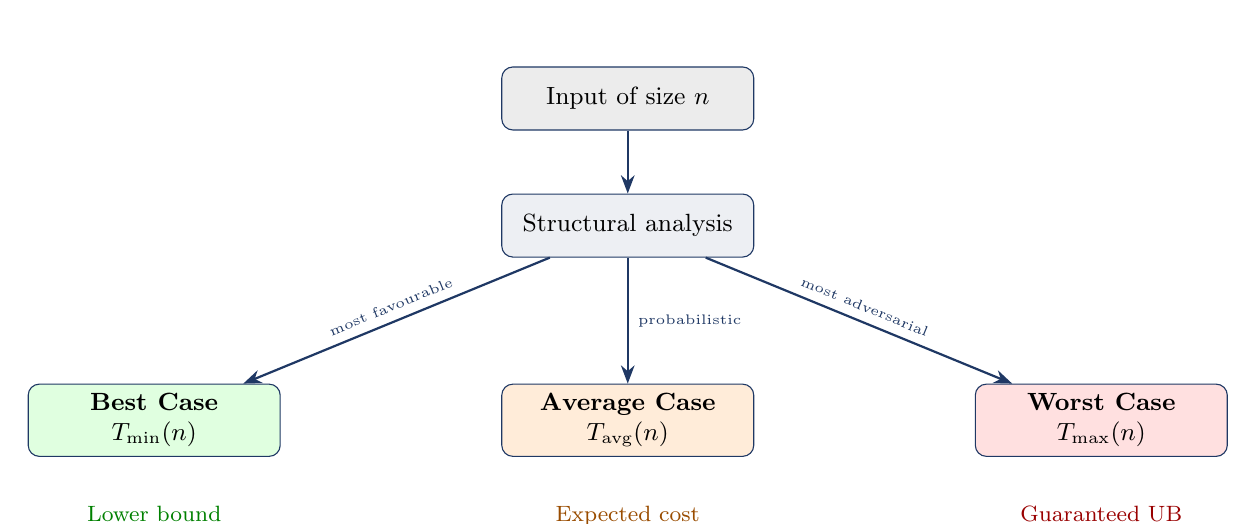
\begin{tikzpicture}[
  node distance=8mm and 24mm,
  box/.style={draw=upesnavy,rounded corners=4pt,fill=upesnavy!8,
              minimum width=32mm,minimum height=8mm,font=\small,align=center},
  arr/.style={-Stealth,thick,upesnavy}]

\node[box,fill=gray!15]               (inp)  {Input of size $n$};
\node[box,below=of inp]               (chk)  {Structural analysis};
\node[box,fill=green!12, below left=16mm and 28mm of chk]  (bc) {\textbf{Best Case}\\$T_{\min}(n)$};
\node[box,fill=orange!15,below=16mm of chk]                (ac) {\textbf{Average Case}\\$T_{\text{avg}}(n)$};
\node[box,fill=red!12,  below right=16mm and 28mm of chk]  (wc) {\textbf{Worst Case}\\$T_{\max}(n)$};

\node[font=\footnotesize,below=5mm of bc,text=green!50!black] {Lower bound};
\node[font=\footnotesize,below=5mm of ac,text=orange!60!black]{Expected cost};
\node[font=\footnotesize,below=5mm of wc,text=red!60!black]   {Guaranteed UB};

\draw[arr] (inp)--(chk);
\draw[arr] (chk)--node[above,sloped,font=\tiny]{most favourable}(bc);
\draw[arr] (chk)--node[right,font=\tiny]{probabilistic}(ac);
\draw[arr] (chk)--node[above,sloped,font=\tiny]{most adversarial}(wc);
\end{tikzpicture}
\caption{Three cases arising from the same input size $n$. Each represents a
different set of input configurations; together they bound and characterise the
full performance envelope of an algorithm.}
\label{fig:intuition}
\end{figure}

%======================== 3 MATHEMATICS ========================
\section{Mathematical Formulation}

Let $\mathcal{I}_n$ denote the set of all valid inputs of size $n$. For any given
input $I \in \mathcal{I}_n$, let $T(I)$ be the number of primitive operations (such
as comparisons, assignments, or swaps) executed by algorithm $\mathcal{A}$.

\subsection{Best-Case Complexity}
\begin{equation}
  T_{\text{best}}(n) = \min_{I\,\in\,\mathcal{I}_n} T(I)
  \label{eq:best}
\end{equation}
Equation~\eqref{eq:best} defines the absolute minimum work an algorithm can do on an
input of size $n$. While it shows whether an early-exit optimization works, it rarely
provides a practical guarantee for everyday inputs.

\subsection{Worst-Case Complexity}
\begin{equation}
  T_{\text{worst}}(n) = \max_{I\,\in\,\mathcal{I}_n} T(I)
  \label{eq:worst}
\end{equation}
Equation~\eqref{eq:worst} gives an upper bound guarantee: no matter what input of
size $n$ we feed into the program, it will never execute more than $T_{\text{worst}}(n)$
operations. Because of this certainty, engineers rely on worst-case bounds for
safety-critical systems~\cite{cormen2022}.

\subsection{Average-Case Complexity}
If $P(I)$ is the probability of receiving a specific input $I$, with
$\sum_{I\in\mathcal{I}_n}P(I)=1$, the expected running time is given by:
\begin{equation}
  T_{\text{avg}}(n)
    = \mathbb{E}[T]
    = \sum_{I\,\in\,\mathcal{I}_n} P(I)\cdot T(I)
  \label{eq:avg}
\end{equation}
Assuming every permutation of $n$ elements is equally likely to occur, we get the
uniform distribution formula:
\begin{equation}
  T_{\text{avg}}(n) = \frac{1}{n!}\sum_{I\,\in\,\mathcal{I}_n} T(I)
  \label{eq:avguniform}
\end{equation}

\subsection{Notation vs. Case: Avoiding Common Confusion}
A frequent conceptual mistake in DAA is treating asymptotic notations ($O$, $\Omega$,
$\Theta$) as direct synonyms for worst, best, and average cases. As shown in
Table~\ref{tab:notation}, they answer two completely different questions.

\begin{table}[h]
\centering
\begin{tabular}{@{}lll@{}}
\toprule
\textbf{Concept}         & \textbf{What it answers}              & \textbf{Example} \\
\midrule
Best / Worst / Avg case  & \emph{Which inputs are we evaluating?}& Worst case of Quick Sort \\
$O$, $\Omega$, $\Theta$  & \emph{What bound applies to $T(n)$?}  & $\Theta(n^2)$ \\
\midrule
\multicolumn{3}{l}{\footnotesize $\Rightarrow$~Worst-case time of Quick Sort is simultaneously $O(n^2)$, $\Omega(n^2)$,
and $\Theta(n^2)$.}\\
\multicolumn{3}{l}{\footnotesize $\Rightarrow$~Best-case time of Quick Sort is $\Theta(n\log n)$.
Saying ``Big-$O$ = worst case'' is \textbf{incorrect}.}\\
\bottomrule
\end{tabular}
\caption{Asymptotic notation and input cases are orthogonal dimensions. Any
notation can be applied to any case.}
\label{tab:notation}
\end{table}

Figure~\ref{fig:growth} plots the three dominant growth functions that appear in
our analysis: $n$, $n\log n$, and $n^2$.

\begin{figure}[h]
\centering
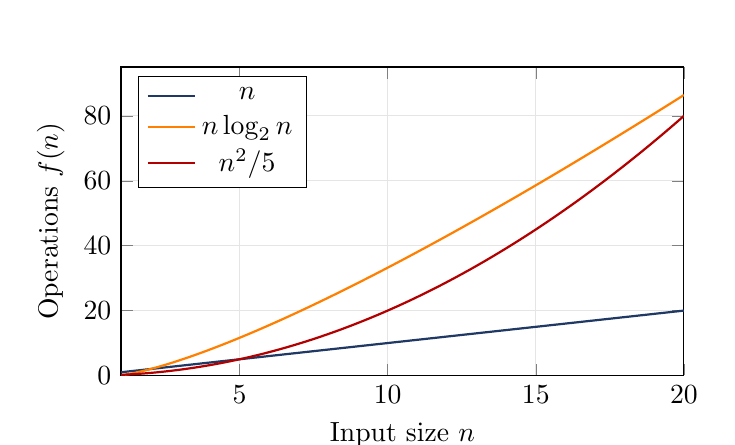
\begin{tikzpicture}
\begin{axis}[width=0.72\linewidth,height=5.5cm,
  xlabel={Input size $n$},ylabel={Operations $f(n)$},
  legend pos=north west,grid=major,grid style={gray!20},
  domain=1:20,samples=80,xmin=1,xmax=20,ymin=0]
\addplot[upesnavy,thick]{x};               \addlegendentry{$n$}
\addplot[orange,thick]{x*ln(x)/ln(2)};     \addlegendentry{$n\log_2 n$}
\addplot[red!70!black,thick]{x^2/5};       \addlegendentry{$n^2/5$}
\end{axis}
\end{tikzpicture}
\caption{Growth rates of $n$, $n\log n$, and $n^2$. Linear Search and Insertion
Sort (best case) run in $\Theta(n)$; Quick Sort (average) in $\Theta(n\log n)$;
Insertion Sort (worst/average) and Quick Sort (worst) in $\Theta(n^2)$.}
\label{fig:growth}
\end{figure}

%======================== 4 ALGORITHM ========================
\section{Algorithm / Procedure}

\subsection{Linear Search}
\begin{algorithm}[H]
\caption{LinearSearch($A$, $n$, $k$)}
\KwIn{Array $A[0\ldots n{-}1]$, integer $n$, target key $k$}
\KwOut{Index $i$ with $A[i]=k$, or $-1$ if absent}
\For{$i \leftarrow 0$ \KwTo $n-1$}{
  \If{$A[i] = k$}{\Return $i$\;}
}
\Return $-1$\;
\end{algorithm}

\subsection{Insertion Sort}
\begin{algorithm}[H]
\caption{InsertionSort($A$, $n$)}
\KwIn{Array $A[0\ldots n{-}1]$}
\KwOut{$A$ sorted in non-decreasing order (in place)}
\For{$j \leftarrow 1$ \KwTo $n-1$}{
  $\mathit{key} \leftarrow A[j]$\;
  $i \leftarrow j-1$\;
  \While{$i \geq 0$ \textbf{and} $A[i] > \mathit{key}$}{
    $A[i+1] \leftarrow A[i]$\;
    $i \leftarrow i-1$\;
  }
  $A[i+1] \leftarrow \mathit{key}$\;
}
\end{algorithm}

\subsection{Quick Sort (overview)}
\begin{algorithm}[H]
\caption{QuickSort($A$, \textit{lo}, \textit{hi})}
\KwIn{Array $A$, indices \textit{lo}, \textit{hi}}
\If{\textit{lo} $<$ \textit{hi}}{
  $\pi \leftarrow \text{Partition}(A,\textit{lo},\textit{hi})$
  \tcp*{$\Theta(n)$ work at each level}
  \text{QuickSort}$(A,\textit{lo},\pi-1)$\;
  \text{QuickSort}$(A,\pi+1,\textit{hi})$\;
}
\end{algorithm}

Core Python excerpt (full source in the repository):
\begin{lstlisting}[language=Python]
def insertion_sort(A):
    for j in range(1, len(A)):
        key = A[j]
        i = j - 1
        while i >= 0 and A[i] > key:   # inner loop: shift right
            A[i + 1] = A[i]
            i -= 1
        A[i + 1] = key                  # insert key at correct position
    return A
\end{lstlisting}

%======================== 5 WORKED EXAMPLE ========================
\section{Worked Example (Step by Step)}

\subsection{Linear Search on $A=[3,7,1,9,4]$, key $=9$}
This traces the \emph{average case}: the key is present at index~3.

\begin{table}[h]
\centering
\begin{tabular}{@{}cccc@{}}
\toprule
\textbf{Step} & \textbf{Index $i$} & \textbf{$A[i]$} & \textbf{Action} \\
\midrule
1 & 0 & 3 & $3\neq 9$ (no match, increment index) \\
2 & 1 & 7 & $7\neq 9$ (no match, increment index) \\
3 & 2 & 1 & $1\neq 9$ (no match, increment index) \\
4 & 3 & 9 & $9=9$ (\textbf{match found; return index 3}) \\
\bottomrule
\end{tabular}
\caption{Linear Search trace: 4 comparisons. Expected value $\frac{n+1}{2}=3$ for
$n=5$, $p=1$. This run is slightly above average, consistent with a random position.}
\end{table}

\subsection{Insertion Sort on $A=[5,3,4,1,2]$}
This traces the \emph{average / general case}.

\begin{table}[h]
\centering
\begin{tabular}{@{}clll@{}}
\toprule
\textbf{Pass $j$} & \textbf{Key} & \textbf{Array before pass} & \textbf{Array after pass} \\
\midrule
1 & 3 & $[5,\ 3,\ 4,\ 1,\ 2]$ & $[3,\ 5,\ 4,\ 1,\ 2]$ \quad (1 shift) \\
2 & 4 & $[3,\ 5,\ 4,\ 1,\ 2]$ & $[3,\ 4,\ 5,\ 1,\ 2]$ \quad (1 shift) \\
3 & 1 & $[3,\ 4,\ 5,\ 1,\ 2]$ & $[1,\ 3,\ 4,\ 5,\ 2]$ \quad (3 shifts) \\
4 & 2 & $[1,\ 3,\ 4,\ 5,\ 2]$ & $[1,\ 2,\ 3,\ 4,\ 5]$ \quad (3 shifts) \\
\bottomrule
\end{tabular}
\caption{Insertion Sort trace: total 8 shifts. The number of inversions in
$[5,3,4,1,2]$ is also 8, which confirms that each shift eliminates exactly one inversion.}
\end{table}

\textbf{Inversion count verification.} The pairs $(i,j)$ with $i<j$ and
$A[i]>A[j]$ in the original array are:
$(5,3),(5,4),(5,1),(5,2),(3,1),(3,2),(4,1),(4,2)$, which gives exactly 8 inversions. \hfill$\square$

%======================== 6 ANIMATION ========================
\section{Animation / Software Demonstration}

To demonstrate these concepts visually, I built an interactive animation using Python and Matplotlib.

\textbf{Tool used:} Python 3, \texttt{matplotlib} (interactive widgets and patches)\\
\textbf{Repository link:} \url{\animationlink}\\
\textbf{How to run:}
\begin{enumerate}
  \item Install dependencies: \texttt{pip install -r requirements.txt}
  \item Run the program: \texttt{python animation.py}
\end{enumerate}
\textbf{Controls available to the user:}
\begin{itemize}
  \item \textbf{Next and Prev buttons}: Step forward or backward through each comparison and shift.
  \item \textbf{Reset button}: Jump back to the initial unsorted state at any time.
  \item \textbf{Best, Avg, and Worst radio buttons}: Switch the input configuration dynamically.
  \item \textbf{Linear Search and Insertion Sort radio buttons}: Switch between the two algorithms.
\end{itemize}

Instead of performing expensive re-calculations on every button click, the script pre-computes each step into an explicit list of program states. Each state records the array contents, which bars to highlight, the step explanation label, and the updated comparison and shift counters.

\begin{figure}[h]
\centering
\begin{subfigure}{0.24\linewidth}\frameimg{figures/frame1.png}
  \caption{Initial array}\end{subfigure}\hfill
\begin{subfigure}{0.24\linewidth}\frameimg{figures/frame2.png}
  \caption{First comparison}\end{subfigure}\hfill
\begin{subfigure}{0.24\linewidth}\frameimg{figures/frame3.png}
  \caption{Shift in progress}\end{subfigure}\hfill
\begin{subfigure}{0.24\linewidth}\frameimg{figures/frame4.png}
  \caption{Sorted complete}\end{subfigure}
\caption{Key frames from the animation. Frame~(a) shows the unsorted array in
blue. Frame~(b) highlights the first comparison in orange. Frame~(c) shows an
element (purple) being shifted during Insertion Sort. Frame~(d) shows the fully
sorted array in green with the final operation count.}
\label{fig:frames}
\end{figure}

%======================== 7 ANALYSIS ========================
\section{Analysis}

\subsection{Per-Algorithm Case Derivations}

\subsubsection*{Linear Search}
\textbf{Best case.} Key at index 0: one comparison.
$T_{\text{best}}(n)=1=\Theta(1)$.

\textbf{Worst case.} Key absent or at index $n-1$: $n$ comparisons.
$T_{\text{worst}}(n)=n=\Theta(n)$.

\textbf{Average case.} Let $p$ be the probability the key is present.
If present, it is equally likely at any of the $n$ positions:
\begin{equation}
\mathbb{E}[T(n)]
  = \frac{p}{n}\sum_{i=1}^{n}i + n(1-p)
  = \frac{p(n+1)}{2}+n(1-p).
\end{equation}
For $p=1$: $\mathbb{E}[T(n)]=\tfrac{n+1}{2}=\Theta(n)$.

\subsubsection*{Insertion Sort}
\textbf{Best case.} Already sorted; the \texttt{while} condition fails
immediately each pass:
$T_{\text{best}}(n)=\sum_{j=1}^{n-1}1=n-1=\Theta(n)$.

\textbf{Worst case.} Reverse sorted; pass $j$ executes $j$ shifts:
\begin{equation}
T_{\text{worst}}(n)=\sum_{j=1}^{n-1}j=\frac{n(n-1)}{2}=\Theta(n^2).
\end{equation}

\textbf{Average case} (inversion analysis~\cite{knuth1998}). Each shift removes
one inversion. A random permutation has expected inversions
\begin{equation}
\mathbb{E}[\text{inv}]
  = \binom{n}{2}\cdot\frac{1}{2} = \frac{n(n-1)}{4},
\end{equation}
giving $T_{\text{avg}}(n)=\Theta(n^2)$.

\subsubsection*{Quick Sort}
\textbf{Best case.} Balanced pivot; recurrence
$T(n)=2T(n/2)+\Theta(n)$.
By Master Theorem Case~2 ($f(n)=\Theta(n^{\log_2 2})$):
$T_{\text{best}}(n)=\Theta(n\log n)$.

\textbf{Worst case.} Degenerate pivot (e.g.\ sorted array, last-element pivot):
$T(n)=T(n-1)+\Theta(n)$.
Unrolling: $T(n)=c\sum_{i=1}^{n}i=\Theta(n^2)$.

\textbf{Average case.} Under uniform random permutations~\cite{cormen2022}:
$T_{\text{avg}}(n)=2n\ln n+O(n)\approx 1.39\,n\log_2 n=\Theta(n\log n)$.

Figure~\ref{fig:qstree} compares the Quick Sort recursion trees for best and
worst cases.

\begin{figure}[h]
\centering
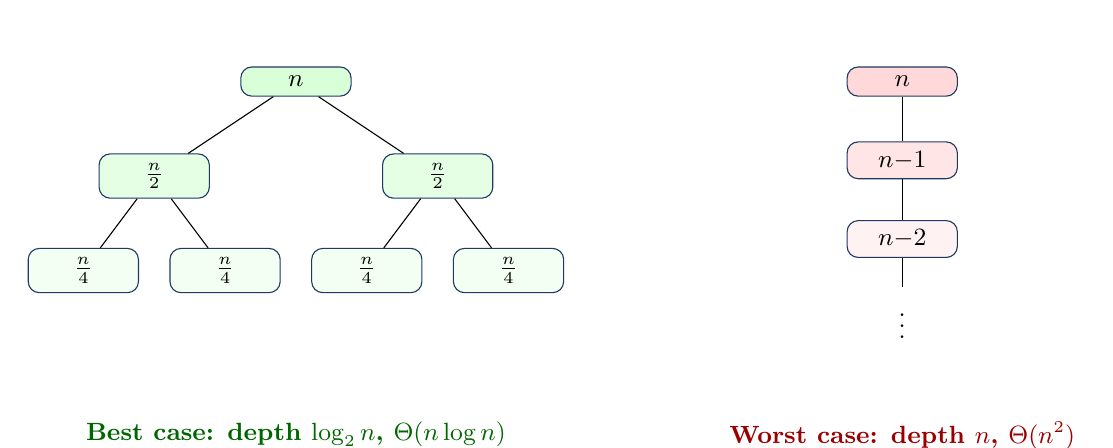
\begin{tikzpicture}[
  level distance=12mm,
  level 1/.style={sibling distance=36mm},
  level 2/.style={sibling distance=18mm},
  every node/.style={draw=upesnavy,rounded corners,fill=upesnavy!8,
                     minimum width=14mm,font=\small,align=center}]
%--- Best case tree (left half) ---
\begin{scope}[xshift=-4.5cm]
\node[fill=green!15] {$n$}
  child{node[fill=green!10]{$\frac{n}{2}$}
    child{node[fill=green!5]{$\frac{n}{4}$}}
    child{node[fill=green!5]{$\frac{n}{4}$}}}
  child{node[fill=green!10]{$\frac{n}{2}$}
    child{node[fill=green!5]{$\frac{n}{4}$}}
    child{node[fill=green!5]{$\frac{n}{4}$}}};
\node[draw=none,fill=none,below=42mm,font=\small\bfseries,text=green!40!black]
  {Best case: depth $\log_2 n$, $\Theta(n\log n)$};
\end{scope}
%--- Worst case tree (right half) ---
\begin{scope}[xshift=3.2cm,level distance=10mm]
\node[fill=red!15] {$n$}
  child[grow=down]{node[fill=red!10]{$n{-}1$}
    child[grow=down]{node[fill=red!5]{$n{-}2$}
      child[grow=down]{node[fill=red!3,draw=none,fill=none]
             {\vdots}}}};
\node[draw=none,fill=none,below=42mm,font=\small\bfseries,text=red!60!black]
  {Worst case: depth $n$, $\Theta(n^2)$};
\end{scope}
\end{tikzpicture}
\caption{Quick Sort recursion trees. The balanced best case (left) has logarithmic
depth; the degenerate worst case (right) degrades to a linear chain, giving
quadratic total work.}
\label{fig:qstree}
\end{figure}

\subsection{Summary Comparison Table}
\begin{table}[h]
\centering
\begin{tabular}{@{}lcccc@{}}
\toprule
\textbf{Algorithm} & \textbf{Best} & \textbf{Average} & \textbf{Worst} & \textbf{Space}\\
\midrule
Linear Search  & $\Omega(1)$       & $\Theta(n)$       & $O(n)$       & $O(1)$ \\
Binary Search  & $\Omega(1)$       & $\Theta(\log n)$  & $O(\log n)$  & $O(1)$ \\
Insertion Sort & $\Omega(n)$       & $\Theta(n^2)$     & $O(n^2)$     & $O(1)$ \\
Merge Sort     & $\Omega(n\log n)$ & $\Theta(n\log n)$ & $O(n\log n)$ & $O(n)$ \\
Quick Sort     & $\Omega(n\log n)$ & $\Theta(n\log n)$ & $O(n^2)$     & $O(\log n)$ \\
Heap Sort      & $\Omega(n\log n)$ & $\Theta(n\log n)$ & $O(n\log n)$ & $O(1)$ \\
\bottomrule
\end{tabular}
\caption{Complexity summary. Merge Sort and Heap Sort achieve $\Theta(n\log n)$
in all cases; Quick Sort matches them on average but degrades to $O(n^2)$ in the
worst case without randomisation.}
\label{tab:comparison}
\end{table}

\subsection{Strengths and Limitations}
\begin{table}[h]
\centering
\begin{tabular}{@{}lll@{}}
\toprule
\textbf{Criterion}    & \textbf{Worst-case analysis}          & \textbf{Average-case analysis} \\
\midrule
Guarantee             & Unconditional upper bound             & Requires input distribution model \\
Practical relevance   & May be overly pessimistic             & Reflects typical runtime \\
Analytical difficulty & Often straightforward                 & Needs combinatorial probability \\
Use case              & Real-time / safety-critical systems   & General-purpose applications \\
\bottomrule
\end{tabular}
\caption{Comparison of worst-case and average-case analysis paradigms.}
\end{table}

%======================== 8 APPLICATIONS ========================
\section{Applications}

\textbf{1. Hard real-time and embedded systems.}
In safety-critical applications like aircraft flight control, automotive anti-lock brakes (ABS), and biomedical pacemakers, computations must finish before strict deadlines. If an algorithm takes even slightly longer than expected, the delay could cause serious physical failure. In these systems, average-case speed is not enough; engineers must design around proven worst-case execution time (WCET) bounds~\cite{kleinberg2006}.

\textbf{2. Guarding against algorithmic complexity attacks (HashDoS).}
When web applications use hash tables with predictable hash functions, an attacker can intentionally craft requests containing keys that all collide into the exact same bucket. This forces lookups to degrade from average $O(1)$ time to worst-case $O(n)$ time, exhausting the server's CPU. To prevent this vulnerability, modern software frameworks use randomized universal hashing, which restores expected $O(1)$ performance regardless of what keys an attacker submits~\cite{cormen2022}.

\textbf{3. Database query optimization.}
Relational databases like PostgreSQL evaluate whether to perform a full sequential scan ($O(n)$) or use an index scan ($O(\log n)$). The query planner uses average-case cost estimations based on table statistics and filter selectivity to pick the most efficient query plan~\cite{sedgewick2011}.

%======================== 9 CONCLUSION ========================
\section{Conclusion}

Studying best, worst, and average case analysis gave me a much clearer perspective on algorithmic trade-offs. The main lesson is that while average-case complexity describes what we encounter most of the time in daily use, worst-case analysis is what guarantees reliability when unusual or adversarial inputs arrive. Furthermore, recognizing that Big-$O$, $\Omega$, and $\Theta$ are mathematical bounding functions rather than synonyms for input cases resolved a common conceptual hurdle.

While creating the step-by-step animation, one observation that stood out was that the number of inner-loop element shifts in Insertion Sort always matches the exact number of inversions in the original input. This clean mathematical connection helped me understand why Insertion Sort runs in $O(n)$ when already sorted, but quickly balloons to $O(n^2)$ when inversions accumulate. A logical next step for exploration would be examining how Shell Sort reduces these inversions across larger gap intervals.

%======================== DECLARATION ========================
\section*{Declaration of AI Tool Use}
\addcontentsline{toc}{section}{Declaration of AI Tool Use}

\noindent\textbf{Tools used:} Google Antigravity (AI assistant)\\
\textbf{Purpose of use:} Assisted with initial LaTeX document setup, table and figure boilerplate, and checking grammar.\\
\textbf{Estimated share of AI-generated content:} Approximately 10--15\% of total assignment effort.\\[4pt]
All mathematical derivations, recurrence solving, algorithm traces, Matplotlib animation code (\texttt{animation.py}), and personal reflections were independently authored, verified, and debugged by me.\\[14pt]
Signature: \rule{4cm}{0.4pt} \hfill Date: \rule{3cm}{0.4pt}

%======================== REFERENCES ========================
\bibliographystyle{ieeetr}
\bibliography{references}

\end{document}
